\documentclass[ddcfooter]{tudbeamer}
\usepackage{german}
\usepackage{graphicx}
\usepackage{caption}
\usepackage{listings}
\usepackage{setspace}
\usepackage{array}

\usetheme{Antibes}


\usepackage{fontspec}
\usepackage{xltxtra}
\setmainfont{Univers}
\setmonofont{Courier}
\setromanfont{Univers}
\setsansfont{Ubuntu}

\begin{document}

\einrichtung{Fakultät Informatik\hspace{6cm} Institut für Systemarchitektur}
\title[Speicherverwaltung in Linux]{Vortrag im Proseminar Betriebssysteme:\vfill Speicherverwaltung in Linux}
\author{Rebecca Kratsch}

\date{10.05.2013}

\maketitle

\section{Inhalt}
\begin{frame}
    \frametitle{Inhalt}
    \begin{itemize}
	\item Grundlegende Konzepte
	\item Verwaltung des physischen Speichers
	\begin{itemize}
	    \item Speicherbelegung am Beispiel des Buddy-Algorithmus
	\end{itemize}
	    \item Repräsentation des virtuellen Speichers
	\begin{itemize}
	    \item Paging
	    \item Seitenersetzungsalgorithmus
	\end{itemize}
    \end{itemize}
\end{frame}



\section{Grundlegendes}
\begin{frame} 
    \frametitle{Grundlegendes}
%     \begin{minipage}[c]{5cm}
%	    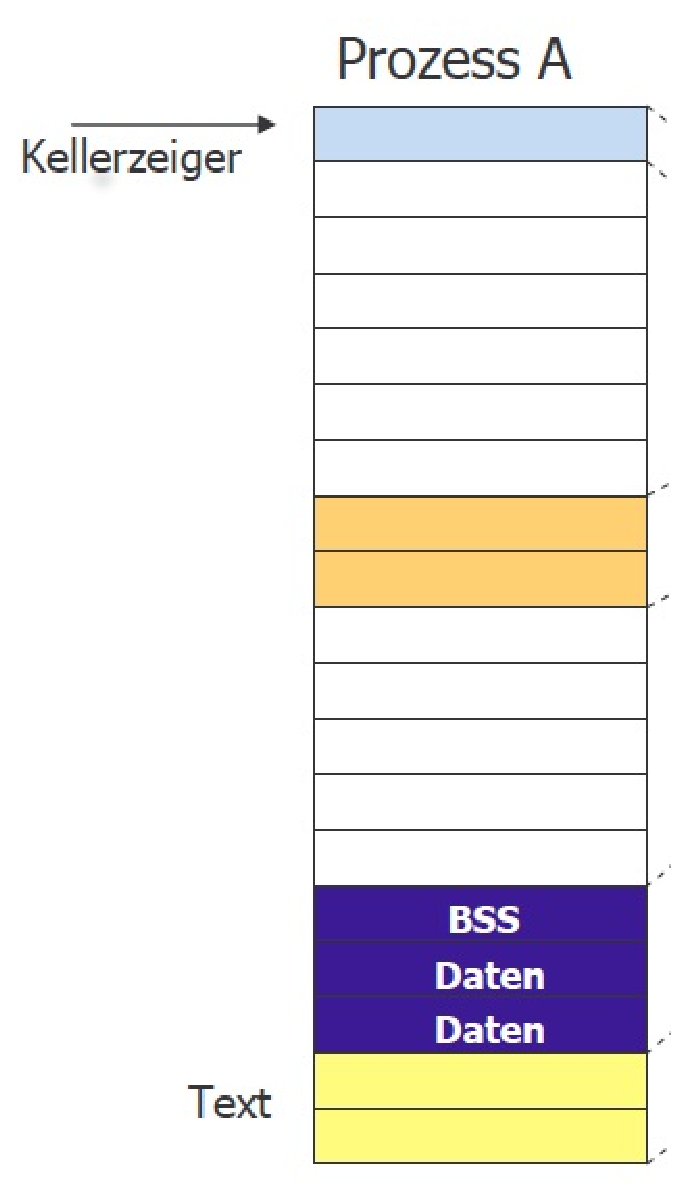
\includegraphics[width = 3cm]{Prozess_A.eps}
%	\end{minipage}
%	\begin{minipage}[c]{5cm}
%	 \begin{tabular}{ l  p{5cm} }
%		Summary \\ 
%		clear day with lots of sunshine.  \\ 
%	    
%	\end{tabular}
%	
%    \end{minipage}
   
\renewcommand{\arraystretch}{1.2}
{\tiny
\begin{tabular}{ | c | c | m{5cm} |}
    	\cline{1-1} \cline{3-3} 
	Stack &  &   \\ \cline{1-1} \cline{3-3}
	      &  &   \\ \cline{1-1} \cline{3-3}               &  &   \\ \cline{1-1} \cline{3-3}
	      &  &   \\ \cline{1-1} \cline{3-3}
	      &  &   \\ \cline{1-1} \cline{3-3}
              &  &   \\ \cline{1-1} \cline{3-3}
	      &  &   \\ \cline{1-1} \cline{3-3}
	      &  &   \\ \cline{1-1} \cline{3-3}
	      &  &   \\ \cline{1-1} \cline{3-3}
	      &  &   \\ \cline{1-1} \cline{3-3}
	      &  &   \\ \cline{1-1} \cline{3-3}
	      &  &   \\ \cline{1-1} \cline{3-3}
	      &  &   \\ \cline{1-1} \cline{3-3}
	      &  &   \\ \cline{1-1} \cline{3-3}
	      &  &   \\ \cline{1-1} \cline{3-3}
	BSS   &  &   \\ \cline{1-1} \cline{3-3} 
	Daten &  &   \\ \cline{1-1} \cline{3-3}    
	Daten &  &   \\ \cline{1-1} \cline{3-3} 
	Text  &  &   \\ \cline{1-1} \cline{3-3}  
	
    \end{tabular}
}
%\renewcommand{\arraystrech}{1}

\end{frame}

\section{virtueller Speicher}
\begin{frame}
    \frametitle{Repräsentation des virtuellen Adressraumes}
    \framesubtitle{Grundlegendes}
    \begin{itemize}
         \item   Unterteilung in homogene, zusammenhängende, an Seitengrenzen ausgerichtete 			Regionen
         \item fixe Seitengröße, erweiterbar durch PAE
         \item Beschreibung jedes Kernbereichs mit \texttt{vm\_area\_struct}-Eintrag 
         \begin{itemize}
         		\item sortiert und zusammengefasst nach virtueller Adresse\\
		\item enthält Eigenschaften (Schutzrechte...)
			--> Realisiserung Copy- on-Write
		\item Angaben über Hintergrundspeicher
    		\item Zugriff auf alle Elemenete eines Adressraumes via Speicher-Deskriptor
		\begin{itemize}
			\item verkette Liste
			\item binärer Rot-Schwarz-Baum
		\end{itemize}
   	\end{itemize} 
     \end{itemize}
    
\end{frame}

\section{virtueller Speicher}
\begin{frame}
    \frametitle{Repräsentation des virtuellen Adressraumes}
    \framesubtitle {Paging in Linux}
    \begin{itemize}
         \item  Grundeinheit: Seite
         \item Grundidee / Definition Paging: \\
        \begin{quote}
         \textquotedblleft
         Paging ist ein Speicherverwaltungsverfahren, das auf der Strukturierung  des virtuellen Speichers 	in Seiten und der Strukturierung des realen Speichers in Seitenrahmen beruht.
    	\textquotedblright \footnote {EHSES, E. u.a. : Betriebssysteme- Ein Lehrbuch mit Übungen zur   	Systemrogrammierung in UNIX/Linux. 3. Aufl. München: Pearson Studium Verlag, 2005, S.294  }
	\end{quote}
 	
	
    
    
     \end{itemize}
    
\end{frame}

\section{virtueller Speicher}
\begin{frame}
    \frametitle{Repräsentation des virtuellen Adressraumes}
    \framesubtitle {Paging in Linux}
    \begin{itemize}
         \item Nutzung 4-stufiger Seitentabellen in Linux
	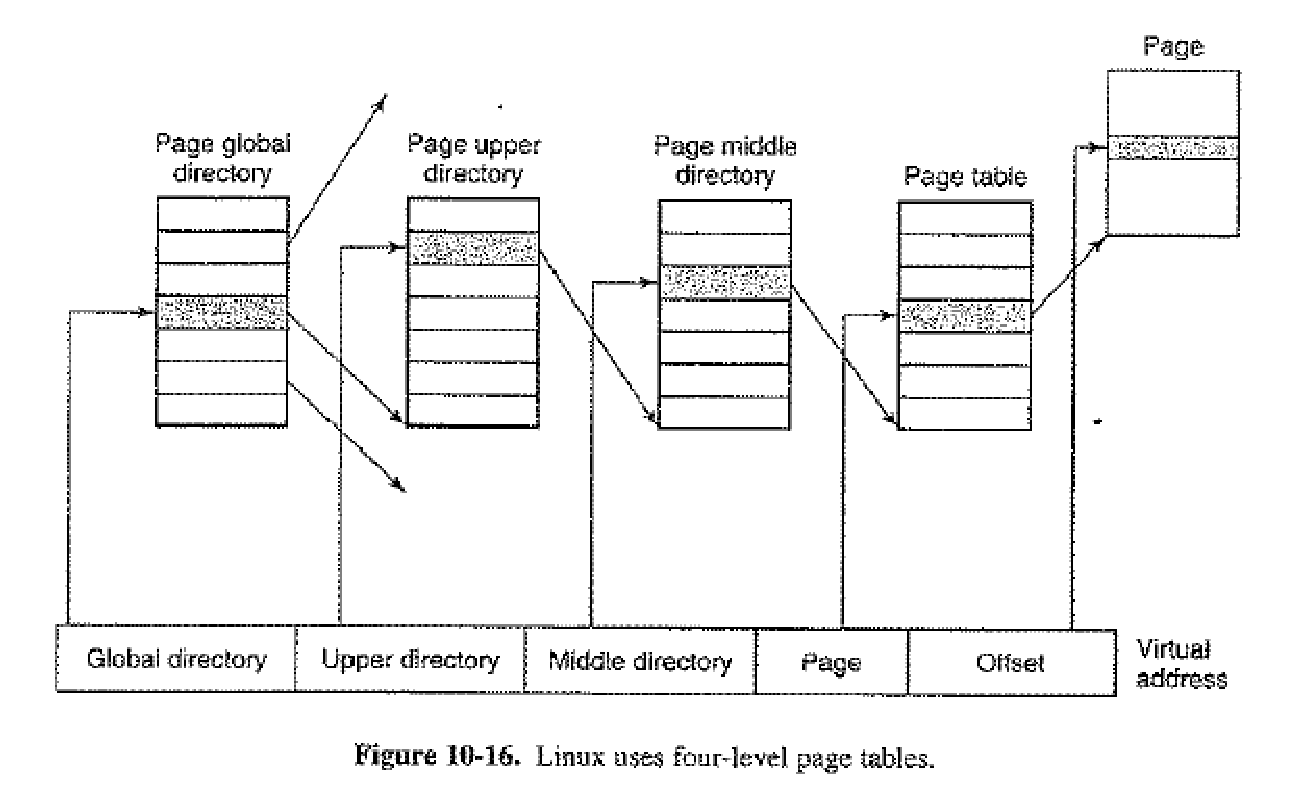
\includegraphics[width=6cm]{Seitentab.eps} 		
    
    
     \end{itemize}
    
\end{frame}

\section{virtueller Speicher}
\begin{frame}
    \frametitle{Repräsentation des virtuellen Adressraumes}
    \framesubtitle {Paging in Linux}
    \begin{itemize}
         \item  Grundeinheit: Seite
         \item Grundidee / Definition Paging: \\
        \begin{quote}
         \textquotedblleft
         Paging ist ein Speicherverwaltungsverfahren, das auf der Strukturierung  des virtuellen Speichers 	in Seiten und der Strukturierung des realen Speichers in Seitenrahmen beruht.
    	\textquotedblright \footnote {EHSES, E. u.a. : Betriebssysteme- Ein Lehrbuch mit Übungen zur   	Systemrogrammierung in UNIX/Linux. 3. Aufl. München: Pearson Studium Verlag, 2005, S.294  }
	\end{quote}
 	 \item Nutzung 4-stufiger Seitentabellen in Linux
	 \item Realisierung sowohl durch kern als auch durch Page-Daemon
	 \item Demand - Paging - System unter Nutzung des Swap-Bereiches
	 \begin{itemize}
	 	\item Auslagerungspartition 
		\item Auslagerungsdateien
	\end{itemize}
    
    
     \end{itemize}
    
\end{frame}


\section{virtueller Speicher}
\begin{frame}
    \frametitle{Repräsentation des virtuellen Adressraumes}
    \framesubtitle {Der Seitenersetzungsalgorithmus}
 
    
\end{frame}



\section{Zusammenfassung}
\begin{frame}
    \frametitle{Zusammenfassung}
    \begin{itemize}
         \item   
    
    
    
     \end{itemize}
    
\end{frame}


\section{Literatur}
\begin{frame}
    \frametitle{Literatur}
    \begin{itemize}
         \item  Moderne Betriebssysteme \\
        		Andrew S. Tanenbaum - 2010
	\item	 UNIX - Wie funktioniert das Betriebssystem? \\
		Maurice J. Bach - 1991
	\item Betriebssysteme\\
		EIn Lehrbuch mit Übungen zur Systemprogrammierung in UNIX/ Linux \\
		E.Ehses, L. Köhler, P. Riemer, H. Stenzel, F. Victor - 2010	
    \end{itemize}
    
\end{frame}

\end{document}






